% !TeX root = ../main.tex
% Add the above to each chapter to make compiling the PDF easier in some editors.

\chapter{Hyperparameter Optimization with Sparse Grids}\label{chapter:main_part}

\section{Methodology}

\subsection{Adaptive Grid Search with Sparse Grids}

\subsection{Implementation}

\section{Results}

\subsection{Experiments with well-defined functions}

Before optimizing the configurations of machine learning models, well defined functions are used. This has the advantage that the optimal point is already known in advance and a function call is much faster than evaluating a neural network. Therefor, three different test functions are given with the following properties \cite{valentin2016hierarchical}:

\begin{table}[htbp!]
		\centering
	\begin{tabular}{|c c c c|} 
		\hline
		Function & Domain & $x_{opt}$ & $ f(x_{opt}) $\\
		\hline
		Eggholder & $[-512, 512]^2 $ & $(512, 404.2319)$ & $ -959.6407 $ \\
		Rosenbrock & $[-5, 10]^2 $ & $(1,1)$ & $ 0 $ \\
		Rastrigin & $[-2, 8]^d $ & $\vec{0}$ & $ 0 $ \\
		\hline
	\end{tabular}
	\caption{ Three test functions and their properties.}
	\label{tab:test_functions}
\end{table}

The plots of the functions can be seen in Figure \ref{fig:test_functions_plot}. The Eggholder function is defined with \cite{whitley1996evaluating} 
\begin{equation}
	f(x_0, x_1) = -x_0 * \text{sin}(\sqrt{ | x_0 - (x_1 + 47) | }) - (x_1 + 47) \text{sin}(\sqrt{ | x_1 +47 + \frac{x_0}{2} | }).
\end{equation}

The second function (Rosenbrock) \cite{yang2010engineering} is calculated with 
\begin{equation}
	f(x_0, x_1) = (1-x_0)^2 + 100 (x_1 - x_0^2)^2.
\end{equation} 
and the third one (Rastrigin) \cite{yang2010engineering} is defined with
\begin{equation}
	f(\vec{x}) = 10 d + \sum_{ i = 1 }^{d} (x_i^2 - 10 \text{cos}(2 \pi x_i))
\end{equation} 
where $ d $ is the dimensionality of the input vector $ \vec{x} $. Figure \ref{fig:test_functions_plot} shows the functions in two dimensions. 


\begin{figure}[htbp!]
	\begin{subfigure}{0.3\textwidth}
		\centering
		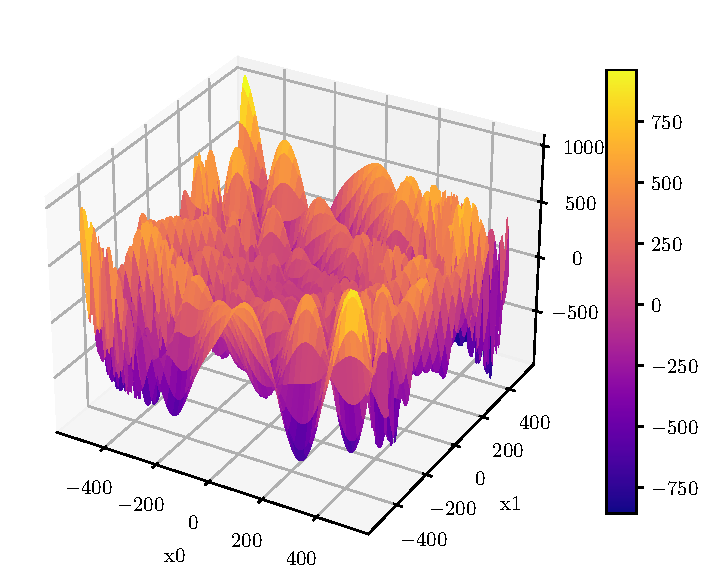
\includegraphics[width=\textwidth]{Eggholder_normal}
		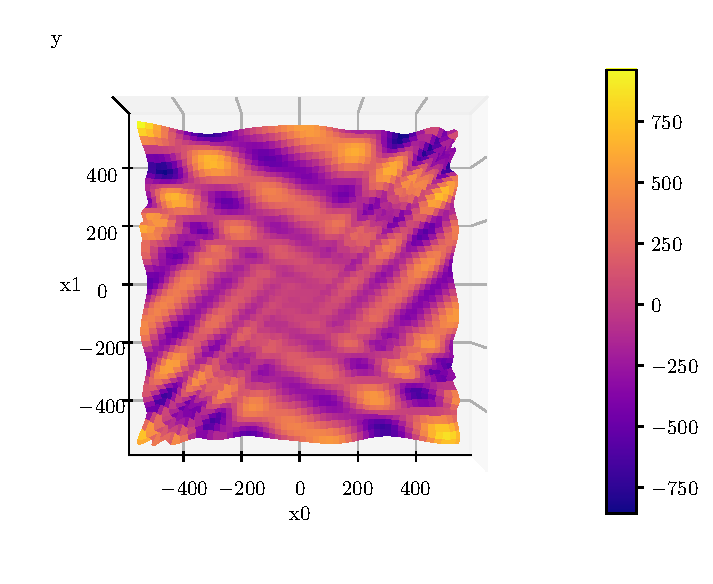
\includegraphics[width=\textwidth]{Eggholder_above}
		\caption{Eggholder.}
		\label{fig:Eggholder}
	\end{subfigure}
	\begin{subfigure}{0.3\textwidth}
		\centering
		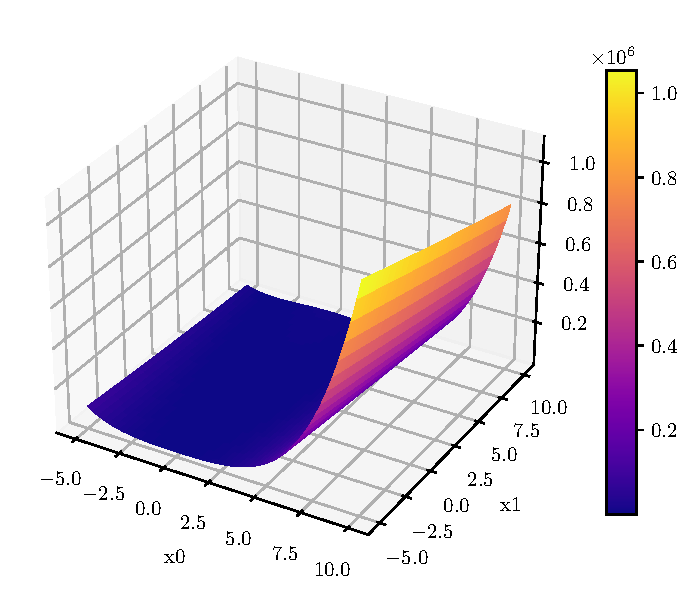
\includegraphics[width=\textwidth]{Rosenbrock_normal}
		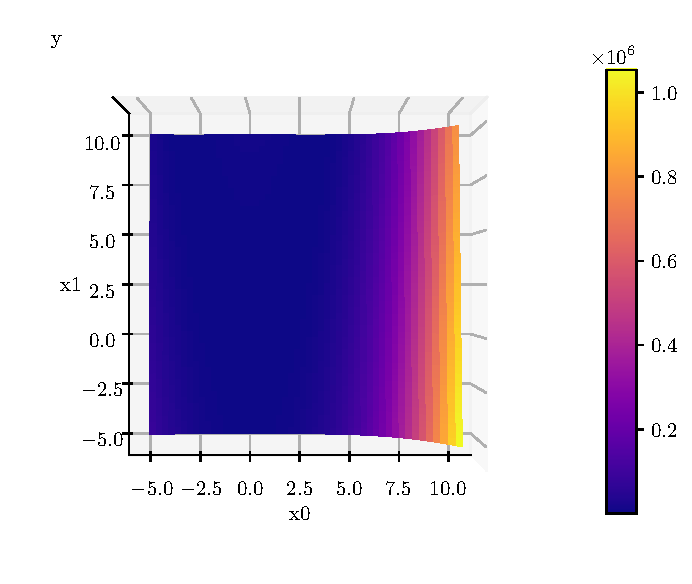
\includegraphics[width=\textwidth]{Rosenbrock_above}
		\caption{Rosenbrock.}
		\label{fig:Rosenbrock}
	\end{subfigure}
	\begin{subfigure}{0.3\textwidth}
		\centering
		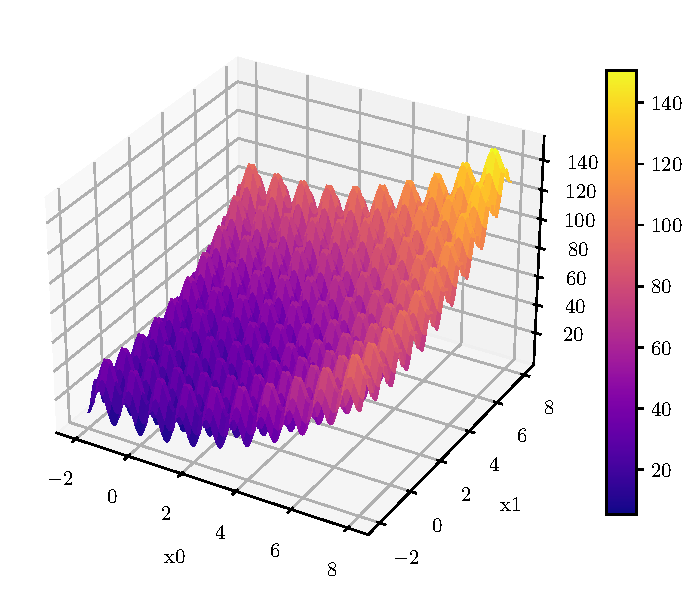
\includegraphics[width=\textwidth]{Rastrigin_normal}
		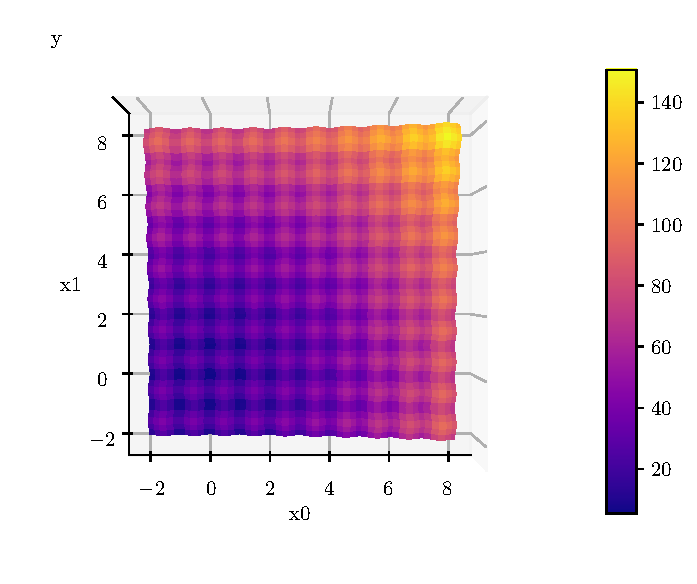
\includegraphics[width=\textwidth]{Rastrigin_above}
		\caption{Rastrigin.}
		\label{fig:Rastrigin}
	\end{subfigure}
	
	\caption{Test functions used for evaluating the Sparse Grid Optimization. Each one is plotted with 200 samples in each dimension.}
	\label{fig:test_functions_plot}
\end{figure}

You can directly see some properties. The Eggholder function (see Figure \ref{fig:Eggholder}) is very oscillatory and the optimal point $ x_{opt} $ lays at the border of the domain. The second one (see Figure \ref{fig:Rosenbrock}) has a big region where the function values are close to the minimum and the last one looks similar (see Figure \ref{fig:Rastrigin}) but with additionally being oscillatory. This might lead to optimizer getting stuck at local minima.

As a first step, we want to concentrate on the sparse grid generation which is done with the Ritter Novak refinement criterion \cite{b_splines}. In each iteration, the grid point $ x_{l,i} $ that minimizes the product 
\begin{equation}
	(r_{l,i} +1)^{1 - \gamma} \cdot (||l||_1 + d_{l,i} + 1)^{\gamma}
\end{equation}
is refined. In this case, $ r_{l,i} = |\{ (l', i') \in K | f(x_{l',i'}) \le f(x_{l,i}) \}| \in \{1, ... , |K|\} $ is the rank of the grid point with $ K $ being the current set of level-index pairs of the grid. Intuitively, this rank denotes the place of the function value in the ascending order of all  values of the current grid. On the other hand, the degree of the point $ d_{l,i} \in \mathbb{N}_0 $ is the number of previous refinements at this point. One important choice is to be made for the adaptivity parameter $ \gamma $. This value has to be between 0 and 1 and the smaller this value is, the more adaptive is the sparse grid. With this value, a trade-off between exploration and exploitation can be balanced. The optimal value depends on the function that has to be optimized.

In the following, the behavior of the sparse grid generation is analyzed with the help of the three test functions. In each case, 3 different values for the adaptivity parameter $ \gamma \in \{0.0, 0.5, 1.0\} $ are used and the resulting sparse grid with the corresponding function values are plotted. The interpolated function is plotted with the triangulation of neighboring grid points. The first test case is the Eggholder function and the result is depicted in Figure \ref{fig:Eggholder_grid}.

\begin{figure}[htbp!]
	\begin{subfigure}{0.3\textwidth}
		\centering
		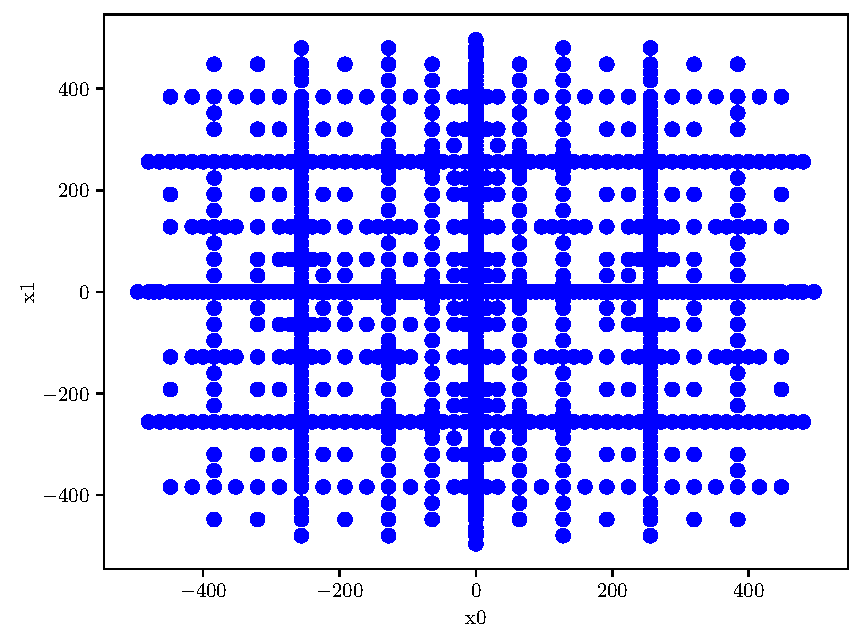
\includegraphics[width=\textwidth]{figures/Results/Sparse_grid_generation_results/Eggholder/tex_files/Eggholder_1}
		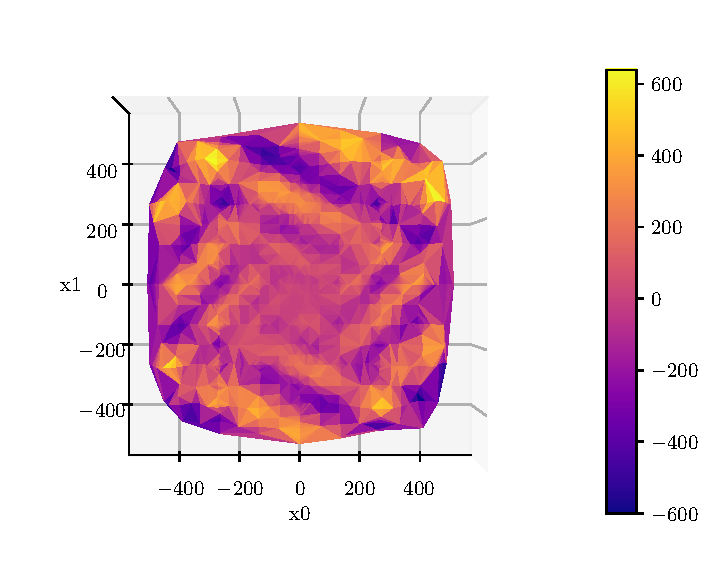
\includegraphics[width=\textwidth]{figures/Results/Sparse_grid_generation_results/Eggholder/tex_files/Eggholder_above_1}
		\caption{$ \gamma = 1.0 $}
		\label{fig:Egg_gamma_1}
	\end{subfigure}
	\begin{subfigure}{0.3\textwidth}
		\centering
		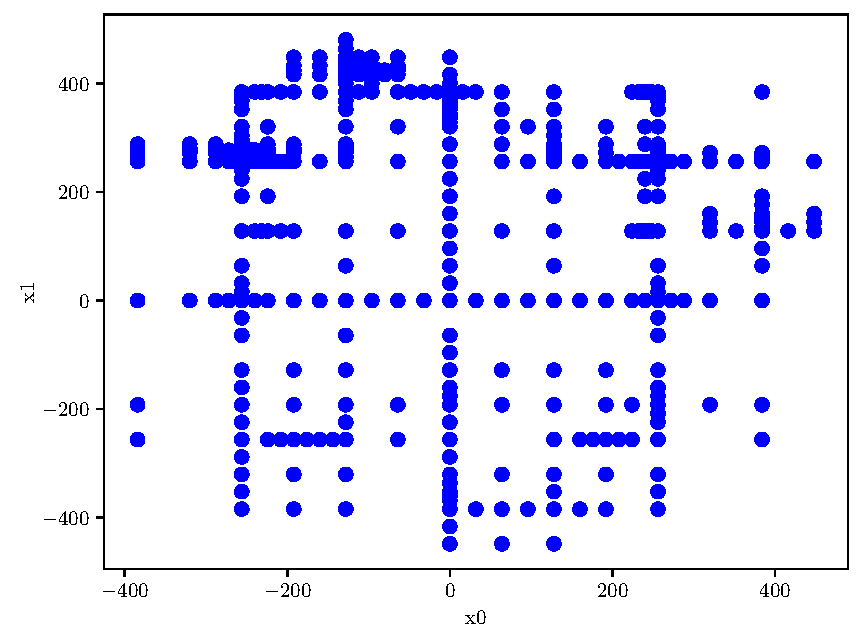
\includegraphics[width=\textwidth]{figures/Results/Sparse_grid_generation_results/Eggholder/tex_files/Eggholder_0_5}
		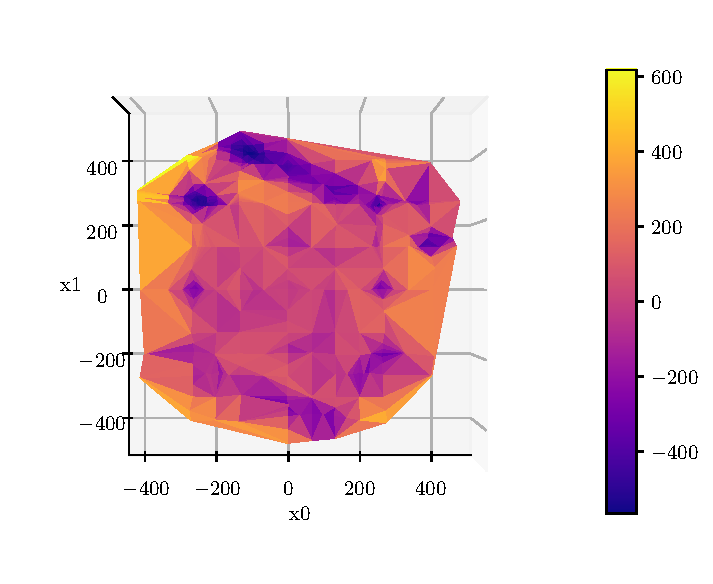
\includegraphics[width=\textwidth]{figures/Results/Sparse_grid_generation_results/Eggholder/tex_files/Eggholder_above_0_5}
		\caption{$ \gamma = 0.5 $}
		\label{fig:Egg_gamma_0_5}
	\end{subfigure}
	\begin{subfigure}{0.3\textwidth}
		\centering
		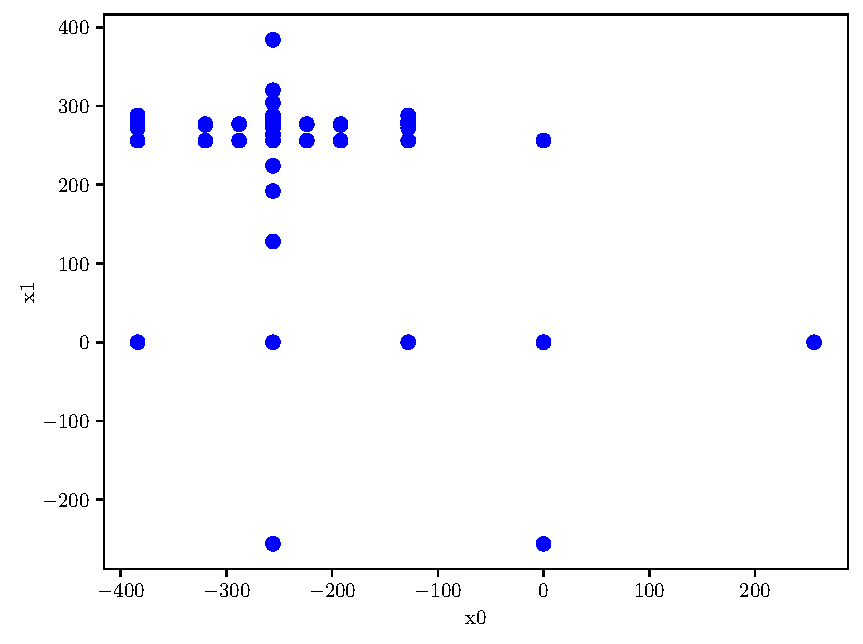
\includegraphics[width=\textwidth]{figures/Results/Sparse_grid_generation_results/Eggholder/tex_files/Eggholder_0}
		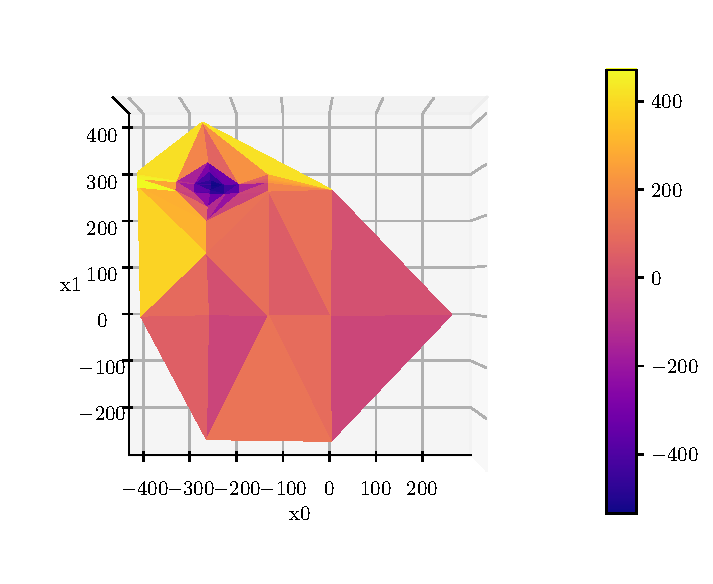
\includegraphics[width=\textwidth]{figures/Results/Sparse_grid_generation_results/Eggholder/tex_files/Eggholder_above_0}
		\caption{$ \gamma = 0.0 $}
		\label{fig:Egg_gamma_0}
	\end{subfigure}
	
	\caption{Sparse grid generation depending on the adaptivity parameter $ \gamma $. In all cases, the same number of grid points is used. Here, in each of the 249 iterations, 4 new grid points are added resulting in a overall number of 997 function evaluations.}
	\label{fig:Eggholder_grid}
\end{figure}

In the first case with $ \gamma = 1.0 $, the grid is homogeneous and not adaptive at all. The function values are distributed over the whole domain and the interpolated function looks very similar to the real plot from Figure \ref{fig:Eggholder}. 

The other extreme case is depicted in Figure \ref{fig:Egg_gamma_0}. There, the grid is maximally adaptive and really concentrated at the top left corner around $ (-260, 280) $. As we know from Table \ref{tab:test_functions}, this is not where the optimal point is located. This behavior can be explained by the high exploitation throughout the iterations. With such a low adaptivity parameter, the points that are low in the first iterations are mostly refined in the other iterations. 

The middle case with $ \gamma = 0.5 $ depicts a case where exploitation and exploration are balanced. The grid points are more distributed than in the case of $ \gamma = 0.0 $ but there are also some regions where the grid points are more defined, e.g. in the top left and right and also around $ (450, -300) $.

Note that in all three cases, the exact same number of grid points are evaluated. In this case it is very hard to find the real optimum because it is located at the border of the domain and the sparse grid does not use grid points at the border. \newline


The next function used is the Rosenbrock function (see Figure \ref{fig:Rosenbrock}). Again, three different values for the adaptivity parameter are used. The results are depicted in Figure \ref{fig:Rosenbrock_grid}.

\begin{figure}[htbp!]
	\begin{subfigure}{0.3\textwidth}
		\centering
		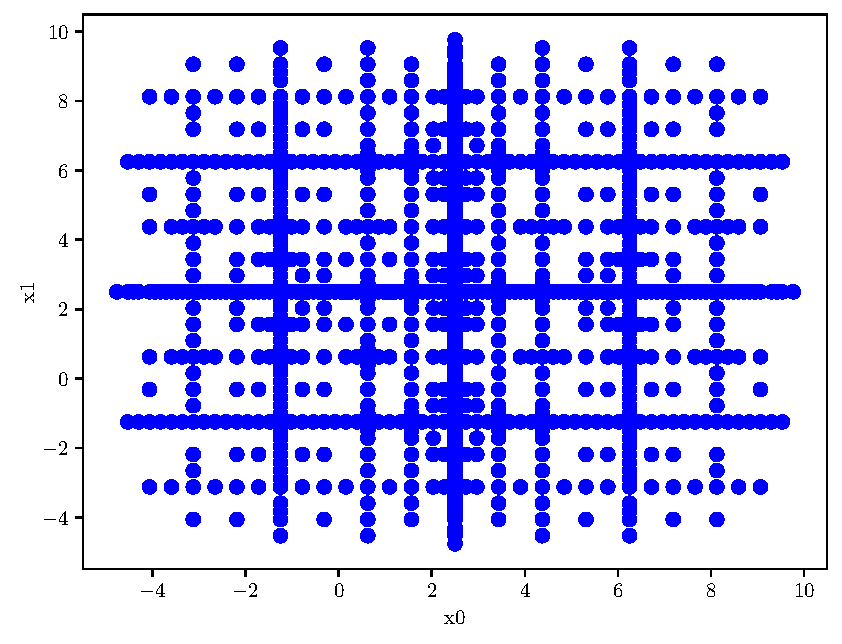
\includegraphics[width=\textwidth]{figures/Results/Sparse_grid_generation_results/Rosenbrock/tex_files/Rosenbrock_1}
		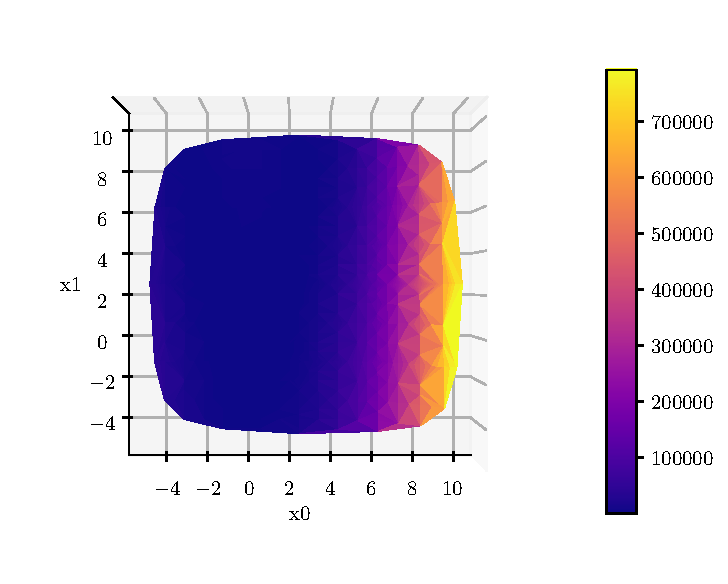
\includegraphics[width=\textwidth]{figures/Results/Sparse_grid_generation_results/Rosenbrock/tex_files/Rosenbrock_above_1}
		\caption{$ \gamma = 1.0 $}
		\label{fig:Ros_gamma_1}
	\end{subfigure}
	\begin{subfigure}{0.3\textwidth}
		\centering
		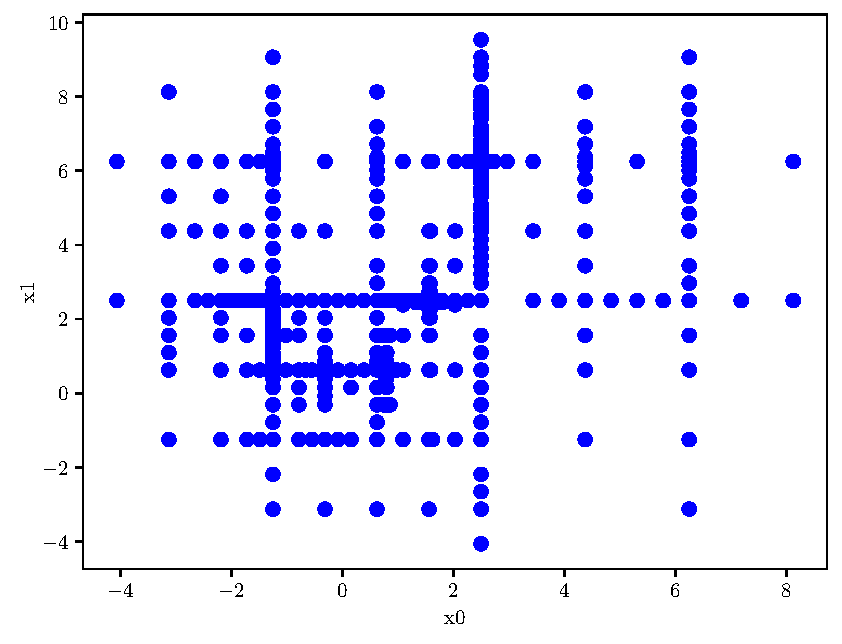
\includegraphics[width=\textwidth]{figures/Results/Sparse_grid_generation_results/Rosenbrock/tex_files/Rosenbrock_0_5}
		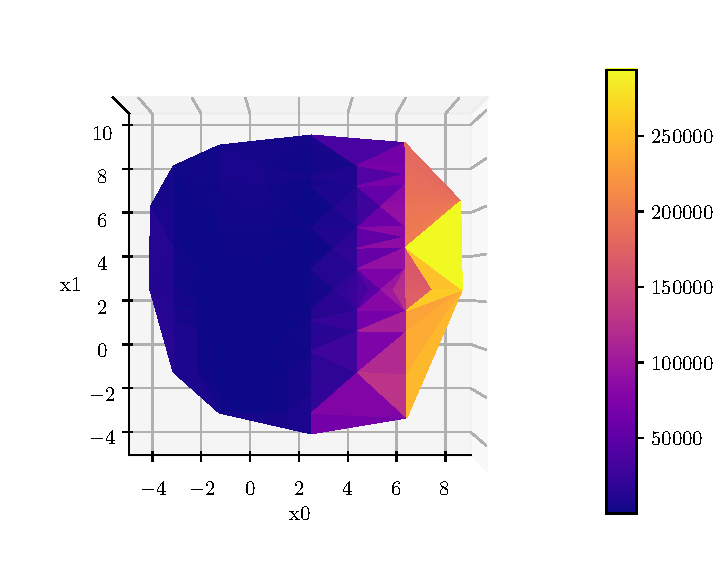
\includegraphics[width=\textwidth]{figures/Results/Sparse_grid_generation_results/Rosenbrock/tex_files/Rosenbrock_above_0_5}
		\caption{$ \gamma = 0.5 $}
		\label{fig:Ros_gamma_0_5}
	\end{subfigure}
	\begin{subfigure}{0.3\textwidth}
		\centering
		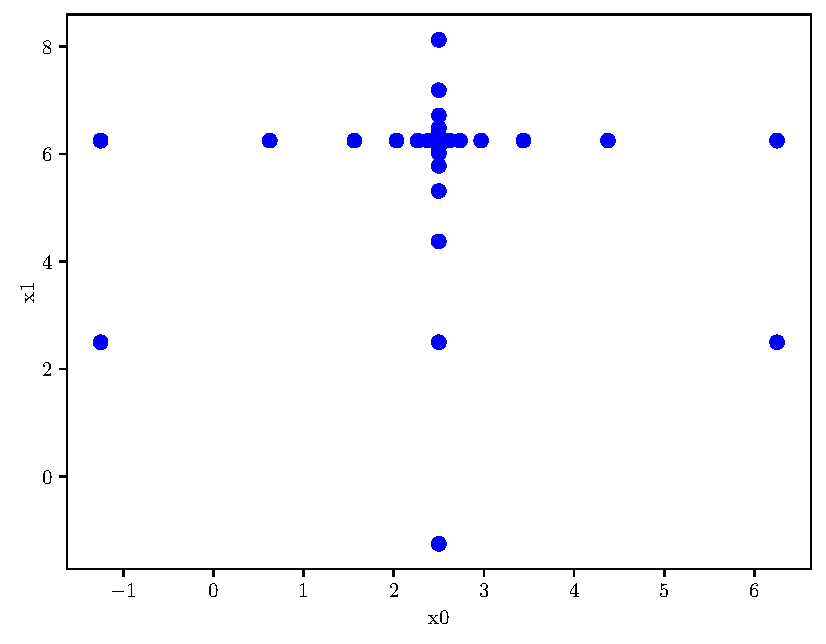
\includegraphics[width=\textwidth]{figures/Results/Sparse_grid_generation_results/Rosenbrock/tex_files/Rosenbrock_0}
		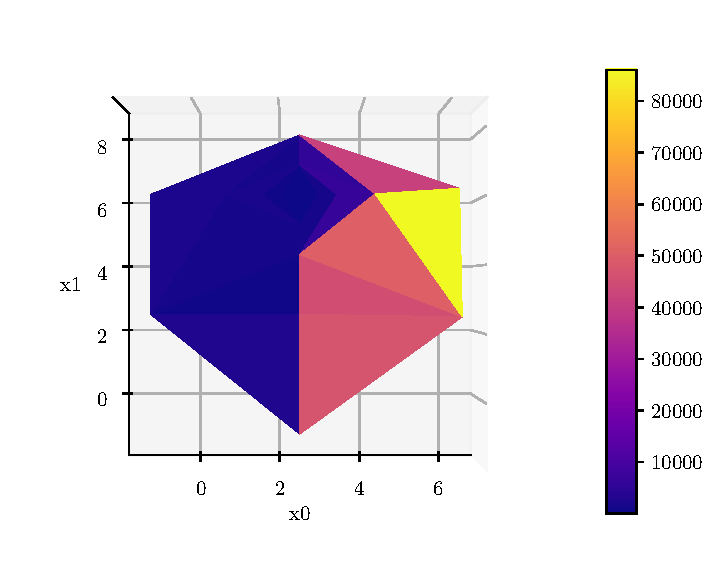
\includegraphics[width=\textwidth]{figures/Results/Sparse_grid_generation_results/Rosenbrock/tex_files/Rosenbrock_above_0}
		\caption{$ \gamma = 0.0 $}
		\label{fig:Ros_gamma_0}
	\end{subfigure}
	
	\caption{Sparse grid generation depending on the adaptivity parameter $ \gamma $. In all cases, the same number of grid points is used. Here, in each of the 249 iterations, 4 new grid points are added resulting in a overall number of 997 function evaluations.}
	\label{fig:Rosenbrock_grid}
\end{figure}


The first fact that can be observed is that the sparse grid in the first case (Figure \ref{fig:Ros_gamma_1}) is exactly the same as the one for the Eggholder function (Figure \ref{fig:Egg_gamma_1}). This is due to the fact that this value of $ \gamma $ leads to a homogeneous sparse grid which is not dependent on the function used but rather the number of iterations for the grid generation. In this case, the interpolated function looks similar to the real function (Figure \ref{fig:Rosenbrock}). 

Now with decreasing value of $ \gamma $, the grid gets more and more inhomogeneous, while concentrating to refine smaller function values. The extreme case can be seen in Figure \ref{fig:Ros_gamma_0}, where the most grid points are next to the point $ (0.65, 0.65) $. This is close to the real optimal point which is located at $ (1, 1) $. \newline 


The last function used is the Rastrigin function (see Figure \ref{fig:Rastrigin} for the plot of the function and \ref{fig:Rastrigin_grid} for the resulting sparse grids). 

\begin{figure}[htbp!]
	\begin{subfigure}{0.3\textwidth}
		\centering
		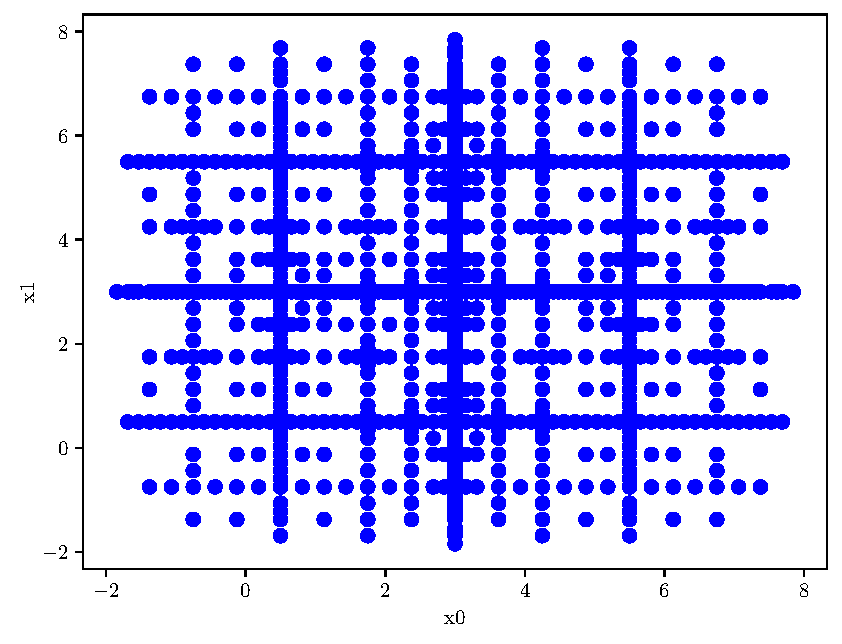
\includegraphics[width=\textwidth]{figures/Results/Sparse_grid_generation_results/Rastrigin/tex_files/Rastrigin_1}
		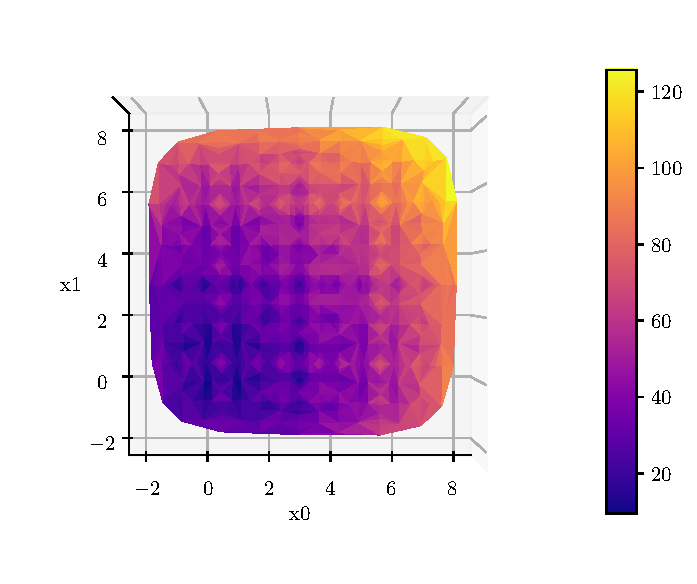
\includegraphics[width=\textwidth]{figures/Results/Sparse_grid_generation_results/Rastrigin/tex_files/Rastrigin_above_1}
		\caption{$ \gamma = 1.0 $}
		\label{fig:Ras_gamma_1}
	\end{subfigure}
	\begin{subfigure}{0.3\textwidth}
		\centering
		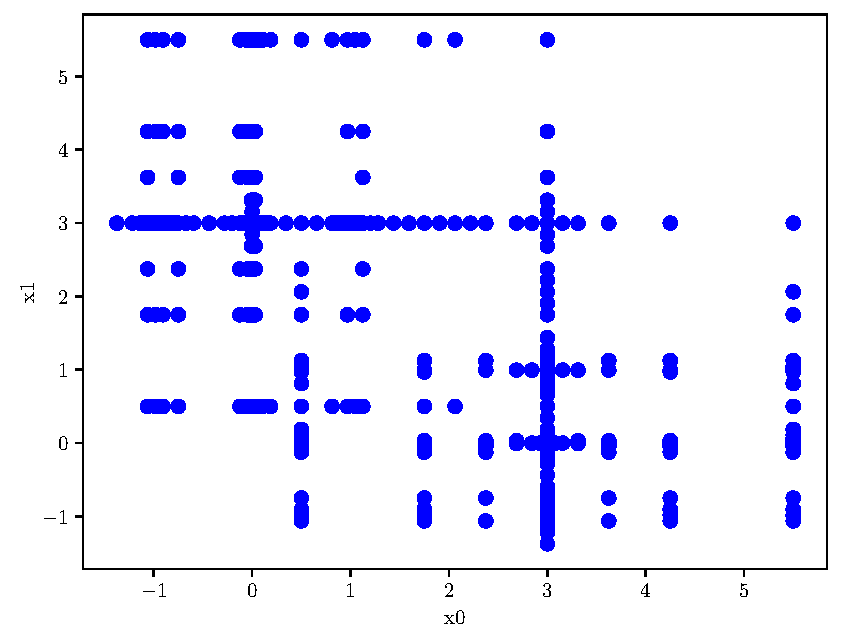
\includegraphics[width=\textwidth]{figures/Results/Sparse_grid_generation_results/Rastrigin/tex_files/Rastrigin_0_5}
		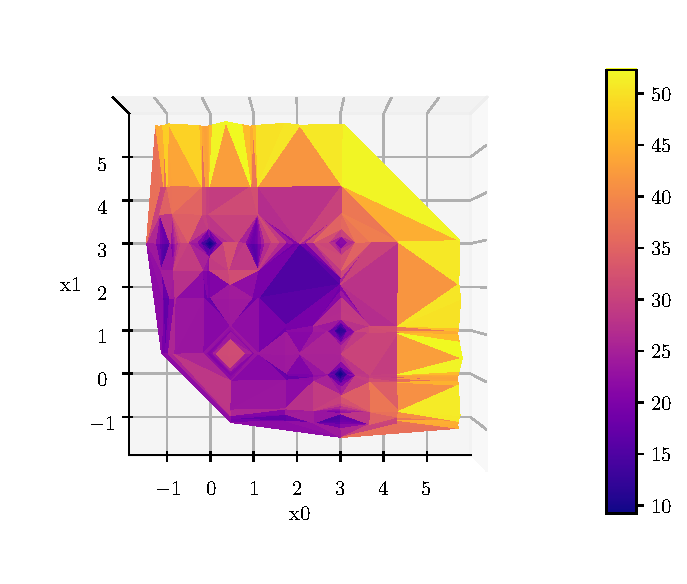
\includegraphics[width=\textwidth]{figures/Results/Sparse_grid_generation_results/Rastrigin/tex_files/Rastrigin_above_0_5}
		\caption{$ \gamma = 0.5 $}
		\label{fig:Ras_gamma_0_5}
	\end{subfigure}
	\begin{subfigure}{0.3\textwidth}
		\centering
		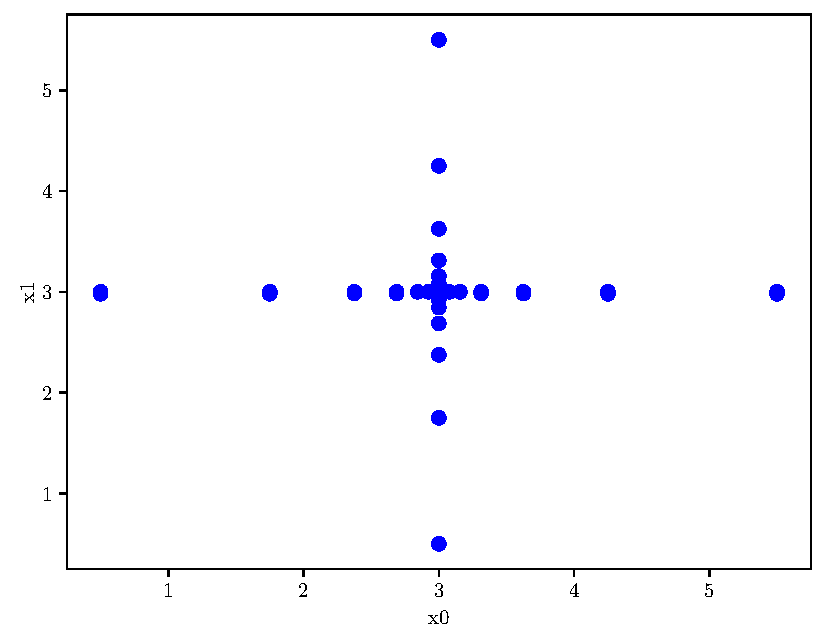
\includegraphics[width=\textwidth]{figures/Results/Sparse_grid_generation_results/Rastrigin/tex_files/Rastrigin_0}
		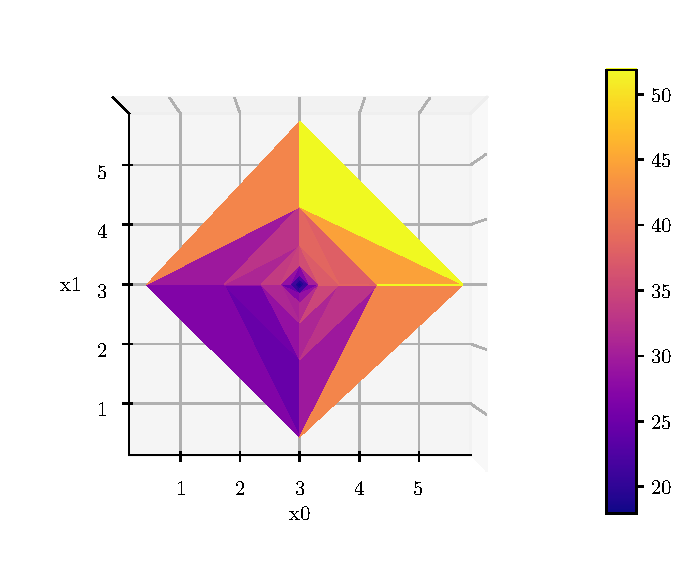
\includegraphics[width=\textwidth]{figures/Results/Sparse_grid_generation_results/Rastrigin/tex_files/Rastrigin_above_0}
		\caption{$ \gamma = 0.0 $}
		\label{fig:Ras_gamma_0}
	\end{subfigure}
	
	\caption{Sparse grid generation depending on the adaptivity parameter $ \gamma $. In all cases, the same number of grid points is used. Here, in each of the 249 iterations, 4 new grid points are added resulting in a overall number of 997 function evaluations.}
	\label{fig:Rastrigin_grid}
\end{figure}

As in the previous two cases, the sparse grid is exactly the same for $ \gamma = 1 $. We can also see the same behavior for a decreasing adaptivity parameter, this time concentrating around the optimal point which is known beforehand $ (0,0) $. \newline 


All in all, these experiments show that the value for the adaptivity parameter strongly influences the grid generation and the resulting optimal value found by the algorithm. In the case of strong oscillatory functions, a rather high value for the adaptivity parameter should be chosen because otherwise, the grid could refine at local optima. In the other cases, we have seen that the grid refines in the correct region for a smaller adaptivity parameter. 

\begin{figure}
		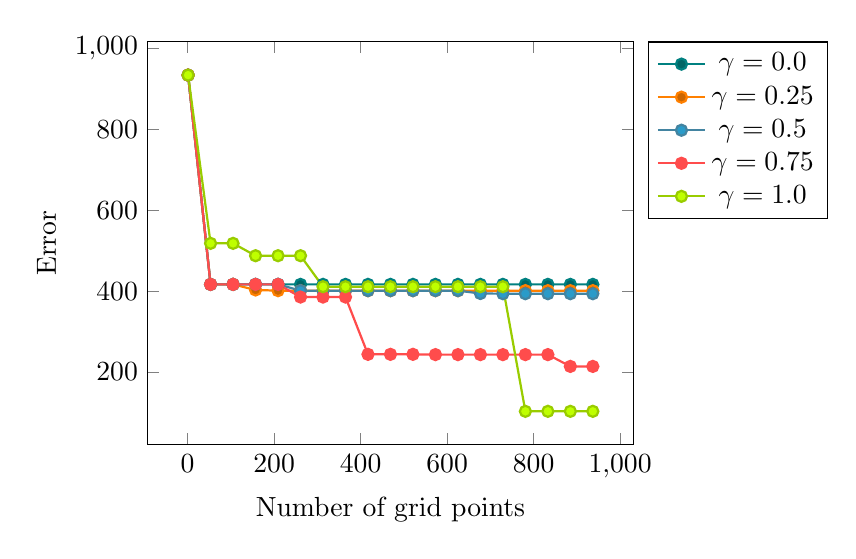
\begin{tikzpicture}
			\begin{axis}[
				xlabel = Number of grid points,
				ylabel = Error,
				scale=0.9,
				cycle list name=exotic,
				legend pos=outer north east,
				]
				
				\addplot+[mark=*, style=thick] coordinates {(1,934.1803628147137)(53,416.6753127436343)(105,416.67517650515606)(157,416.67517650515606)(209,416.6751765051557)(261,416.6751765051555)(313,416.67517650515515)(365,416.67517650515583)(417,416.67517650515606)(469,416.67517650515515)(521,416.67517650515595)(573,416.6751765051555)(625,416.6751765051557)(677,416.6751765051554)(729,416.6751765051555)(781,416.67517650515595)(833,416.6751765051555)(885,416.6751765051557)(937,416.6751765051557)};
				
				\addplot+[mark=*, style=thick]  coordinates 
				{(1,934.1803628147137)(53,416.6753127436343)(105,416.67517650515606)(157,402.86392358909313)(209,401.165066632121)(261,401.16506654901593)(313,401.16506654901764)(365,401.1650665490138)(417,401.1650665490125)(469,401.1650665490105)(521,401.16506654901195)(573,401.1650665490175)(625,401.16506654902184)(677,401.16506654901843)(729,401.16506654901593)(781,401.1650665490224)(833,401.16506654902105)(885,401.1650665490139)(937,401.1650665490138)};
				
				\addplot+[mark=*, style=thick]   coordinates 
				{(1,934.1803628147137)(53,416.6753127436343)(105,416.67517650515595)(157,416.67517650515595)(209,416.6751765051556)(261,401.16506923718293)(313,401.1650665490133)(365,401.1650665490122)(417,401.16506654901445)(469,401.1650665490125)(521,401.16506654901264)(573,401.16506654901264)(625,401.1650665490216)(677,394.1301115312152)(729,393.6496427441624)(781,393.6444455890784)(833,393.6437130885647)(885,393.6437130885688)(937,393.6437130885528)};
				
				\addplot+[mark=*, style=thick]  coordinates
					{(1,934.1803628147137)(53,416.680649645461)(105,416.67519174547897)(157,416.6751765051557)(209,416.6751765051554)(261,385.37674780492864)(313,385.35652906792404)(365,385.3565290679238)(417,243.68003942485666)(469,243.67992321536838)(521,243.67992321536633)(573,243.01108728703605)(625,242.99463717547087)(677,242.99463717547076)(729,242.99463717547087)(781,242.99463717546962)(833,242.99463717546973)(885,213.83490792055488)(937,213.834907133721)};
				
				\addplot+[mark=*, style=thick]  coordinates 
				{(1,934.1803628147137)(53,518.1399491004825)(105,518.1399491004823)(157,487.54622876272015)(209,487.54622876272003)(261,487.54622876272)(313,410.9897867087419)(365,410.9897867087424)(417,410.9897867087427)(469,410.9897867087419)(521,410.9897867087424)(573,410.98978670874214)(625,410.9897867087425)(677,410.9897867087424)(729,410.9897867087428)(781,102.75674102278083)(833,102.7567410227864)(885,102.75674102278651)(937,102.75674102279345)};
			
				\legend{$ \gamma = 0.0 $, $ \gamma = 0.25 $, $ \gamma = 0.5 $, $ \gamma = 0.75 $, $ \gamma = 1.0 $,}
				
			\end{axis}
		\end{tikzpicture}


		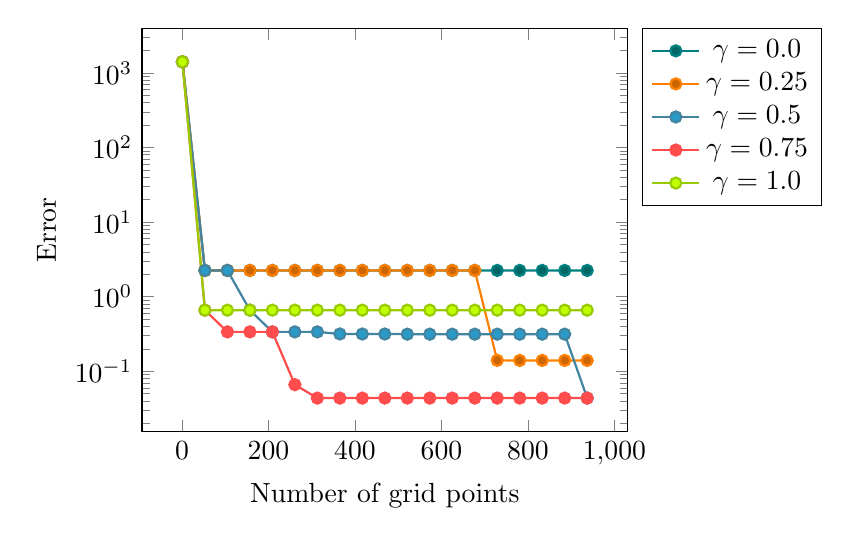
\begin{tikzpicture}
			\begin{axis}[
				xlabel = Number of grid points,
				ylabel = Error,
				scale = 0.9,
				ymode=log,
				cycle list name=exotic,
				legend pos=outer north east,
				]
				
				\addplot+[mark=*, style=thick] coordinates {(1,1408.5)(53,2.25)(105,2.2491001457701714)(157,2.2491001457701714)(209,2.2491001457722626)(261,2.2491001457672675)(313,2.249100145771435)(365,2.249100145769731)(417,2.2491001457715205)(469,2.249100145772637)(521,2.2491001457718287)(573,2.249100145770883)(625,2.2491001457697997)(677,2.24910014577051)(729,2.2491001457706186)(781,2.249100145769841)(833,2.2491001457692894)(885,2.249100145769003)(937,2.2491001457706337)};
				
				\addplot+[mark=*, style=thick]  coordinates 
				{(1,1408.5)(53,2.25)(105,2.2491001457701714)(157,2.2491001457701714)(209,2.2491001457721036)(261,2.2491001457695767)(313,2.249100145770952)(365,2.2491001457690514)(417,2.2491001457697983)(469,2.2491001457687094)(521,2.2491001457707274)(573,2.249100145770689)(625,2.2491001457705138)(677,2.249100145770712)(729,0.13999960097248135)(781,0.13973409018662308)(833,0.1397340901880652)(885,0.1397340901910032)(937,0.13973409019308297)};
				
				\addplot+[mark=*, style=thick]   coordinates 
				{(1,1408.5)(53,2.25)(105,2.2491001457701714)(157,0.65972900390625)(209,0.33738539328720274)(261,0.337384855010467)(313,0.3373848550084554)(365,0.3164062500005624)(417,0.3160824744022442)(469,0.316082474402264)(521,0.3143689789723247)(573,0.31436571579881106)(625,0.3143657157996295)(677,0.3143657157842261)(729,0.3143657158217291)(781,0.31436571578093114)(833,0.3143657158159762)(885,0.31436571582376066)(937,0.04369918730841191)};
				
				\addplot+[mark=*, style=thick]  coordinates
				{(1,1408.5)(53,0.65972900390625)(105,0.33738539328578554)(157,0.3373848550099865)(209,0.33738485500900234)(261,0.06609634402749087)(313,0.04368661484965771)(365,0.043686614913836186)(417,0.043686614861208506)(469,0.04368661485251346)(521,0.04368661485326686)(573,0.04368661485538938)(625,0.04368661485308678)(677,0.043686614838481574)(729,0.04368661486120118)(781,0.04368661488831904)(833,0.043686614839174354)(885,0.04368661486845582)(937,0.04368661486256009)};
				
				\addplot+[mark=*, style=thick]  coordinates 
				{(1,1408.5)(53,0.65972900390625)(105,0.65972900390625)(157,0.65972900390625)(209,0.6597290039064774)(261,0.6597290039068184)(313,0.65972900390625)(365,0.65972900390625)(417,0.65972900390625)(469,0.6597290039065911)(521,0.6597290039067047)(573,0.6597290039064774)(625,0.6597290039064774)(677,0.6597290039067047)(729,0.6597290039067047)(781,0.6597290039064774)(833,0.65972900390625)(885,0.6597290039065911)(937,0.6597290039065911)};
				
				\legend{$ \gamma = 0.0 $, $ \gamma = 0.25 $, $ \gamma = 0.5 $, $ \gamma = 0.75 $, $ \gamma = 1.0 $,}
				
			\end{axis}
		\end{tikzpicture}
	
		
		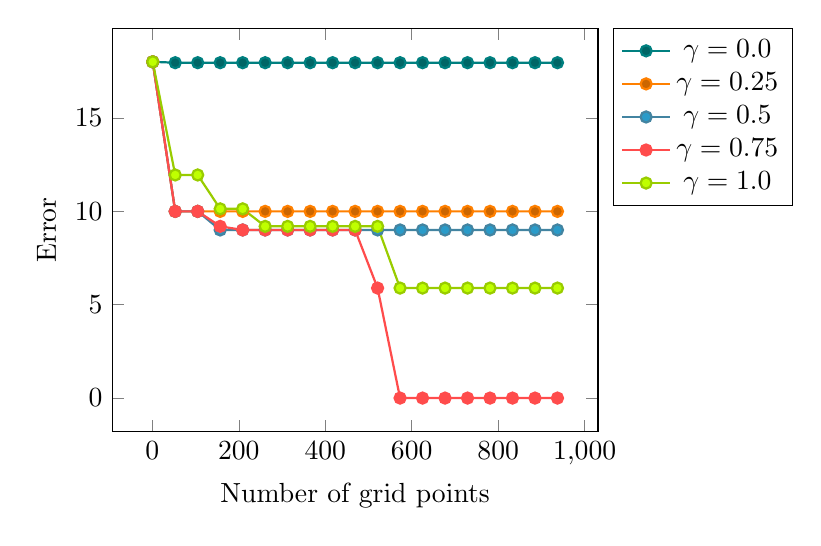
\begin{tikzpicture}
			\begin{axis}[
				xlabel = Number of grid points,
				ylabel = Error,
				scale = 0.9,
				cycle list name=exotic,
				legend pos=outer north east,
				]
				
				\addplot+[mark=*, style=thick] coordinates{(1,18.0)(53,17.954603830243304)(105,17.954601241487484)(157,17.954601241487484)(209,17.95460124148829)(261,17.954601241487573)(313,17.95460124148752)(365,17.954601241487435)(417,17.95460124148751)(469,17.954601241487524)(521,17.954601241487467)(573,17.954601241487463)(625,17.954601241487506)(677,17.954601241487463)(729,17.95460124148793)(781,17.954601241488138)(833,17.954601241487886)(885,17.954601241487513)(937,17.954601241488046)};
				
				\addplot+[mark=*, style=thick]  coordinates 
				{(1,18.0)(53,9.995024358227056)(105,9.994959057644616)(157,9.994959057644616)(209,9.994959057646103)(261,9.99495905764463)(313,9.994959057644524)(365,9.99495905764453)(417,9.99495905764462)(469,9.994959057644579)(521,9.994959057644468)(573,9.994959057644502)(625,9.994959057644628)(677,9.994959057644607)(729,9.99495905764461)(781,9.994959057644595)(833,9.99495905764462)(885,9.994959057644616)(937,9.994959057644667)};
				
				\addplot+[mark=*, style=thick]   coordinates 
				{(1,18.0)(53,9.995024358227056)(105,9.994959057644618)(157,9.000000184767032)(209,9.000000000721773)(261,9.0000000007217)(313,9.000000000721338)(365,9.000000000721721)(417,9.00000000072155)(469,9.00000000072114)(521,9.000000000721972)(573,9.000000000721784)(625,9.00000000072177)(677,9.000000000721762)(729,9.00000000072182)(781,9.000000000721915)(833,9.000000000721828)(885,9.000000000721684)(937,9.000000000721721)};
				
				\addplot+[mark=*, style=thick]  coordinates
				{(1,18.0)(53,9.995597577515051)(105,9.994959320973711)(157,9.193123758467696)(209,9.000000000721291)(261,9.000000000720725)(313,9.00000000073414)(365,9.000000000715445)(417,9.000000000715788)(469,9.00000000072136)(521,5.889114376269022)(573,0.001513592628570368)(625,1.9994962252604298e-07)(677,1.2455895805700494e-08)(729,1.2778394708011167e-08)(781,1.2291804361994243e-08)(833,1.179890717001382e-08)(885,1.251678228282502e-08)(937,1.231146666513552e-08)};
				
				\addplot+[mark=*, style=thick]  coordinates 
				{(1,18.0)(53,11.944557188134524)(105,11.944557188134521)(157,10.130623758467696)(209,10.130623758467692)(261,9.193123758467797)(313,9.193123758467703)(365,9.193123758467696)(417,9.1931237584677)(469,9.1931237584677)(521,9.193123758467692)(573,5.8891143762690925)(625,5.889114376269034)(677,5.88911437626902)(729,5.889114376269047)(781,5.889114376269048)(833,5.889114376269062)(885,5.889114376269007)(937,5.889114376269115)};
				
				\legend{$ \gamma = 0.0 $, $ \gamma = 0.25 $, $ \gamma = 0.5 $, $ \gamma = 0.75 $, $ \gamma = 1.0 $,}
				
			\end{axis}
		\end{tikzpicture}
	
	\caption{$ \gamma = 0.0 $}	
	\label{fig:Functions_results}
\end{figure}

\subsection{Optimization with small neural networks}









